\documentclass{package/fancy-book}

\usepackage[T1]{fontenc}
\usepackage{lmodern}
\usepackage{extarrows}
%%%%%%%%%% Default Package %%%%%%%%%%%%%
\usepackage{package/color-env}
%%%%%%%%%% %%%%%%%%%%%%%%% %%%%%%%%%%%%%
%%%%%%%%%% Required Packages %%%%%%%%%%%%%
\usepackage{background}
\usepackage[object=vectorian]{pgfornament} %% used in title.tex
\usepackage{calligra} %%% (optional) to make the Title text beautiful 
%%%%%%%%%%%%%%%%%%%%%%%%

\usepackage{lipsum}  %% for dummy text 
\usepackage{amssymb,amsmath,amsfonts}  %%% for maths
\usepackage{physics}  %%% for partial derivatives
%%%%%%%%%%%%%%%%%%%%%%%%%%%%%%%%%%%%%

%%%%%% Optional Packages %%%%%%%
\usepackage{lettrine} %% for nice looking 
\usepackage{GoudyIn} %% first Letter of the paragraph

\renewcommand{\LettrineFontHook}{\color{black}\GoudyInfamily{}}
\LettrineTextFont{\itshape}
\setcounter{DefaultLines}{3}%
%%%%%%%%%%%%%%%%%%%%%%%%%%%%%%%%%%%%%
\usepackage{fourier-orns}
\usepackage{tikz}
\usepackage{etoolbox}
\usepackage{enumitem}
\newcommand*{\circled}[1]{\lower.7ex\hbox{\tikz\draw (0pt, 0pt)%
    circle (.5em) node {\makebox[1em][c]{\small #1}};}}
\robustify{\circled}
\newcommand{\ornamento}{\vspace{2em}\noindent \textcolor{darkgray}{\hrulefill~ \raisebox{-2.5pt}[10pt][10pt]{\leafright \decofourleft 
\decothreeleft  \aldineright \decotwo \floweroneleft \decoone   \floweroneright 
\decotwo \aldineleft\decothreeright \decofourright \leafleft} ~  \hrulefill \\ \vspace{2em}}}
%%%% Bibliography %%%%%%%%%
% Required packages are included in notes class
% Can be tweaked in the notes.cls file itself
\newenvironment{solution}{{\par\noindent\it Solution.}}{}
\addbibresource{resource/references.bib}

\begin{document}

\begin{titlepage}

%%%%%%%%%%%%%%%%%%%%%%%%%%%%%%%%%%%% Inspired From  %%%%%%%%%%%%%%%%%%%%%%%%%%%%%%%%%%%%%%%%%%%%%%%%% 
%%%%  https://www.reddit.com/r/LaTeX/comments/j9d739/hello_world_in_latex_is_a_lot_cooler/   %%%%%
%%%%%%%%%%%%%%%% If this doesn't look nice then you may remove it %%%%%%%%%%%%%%%%%%%%%%%%%%

\backgroundsetup{
scale=1,
opacity=1,
angle=0,
color=black,
contents={
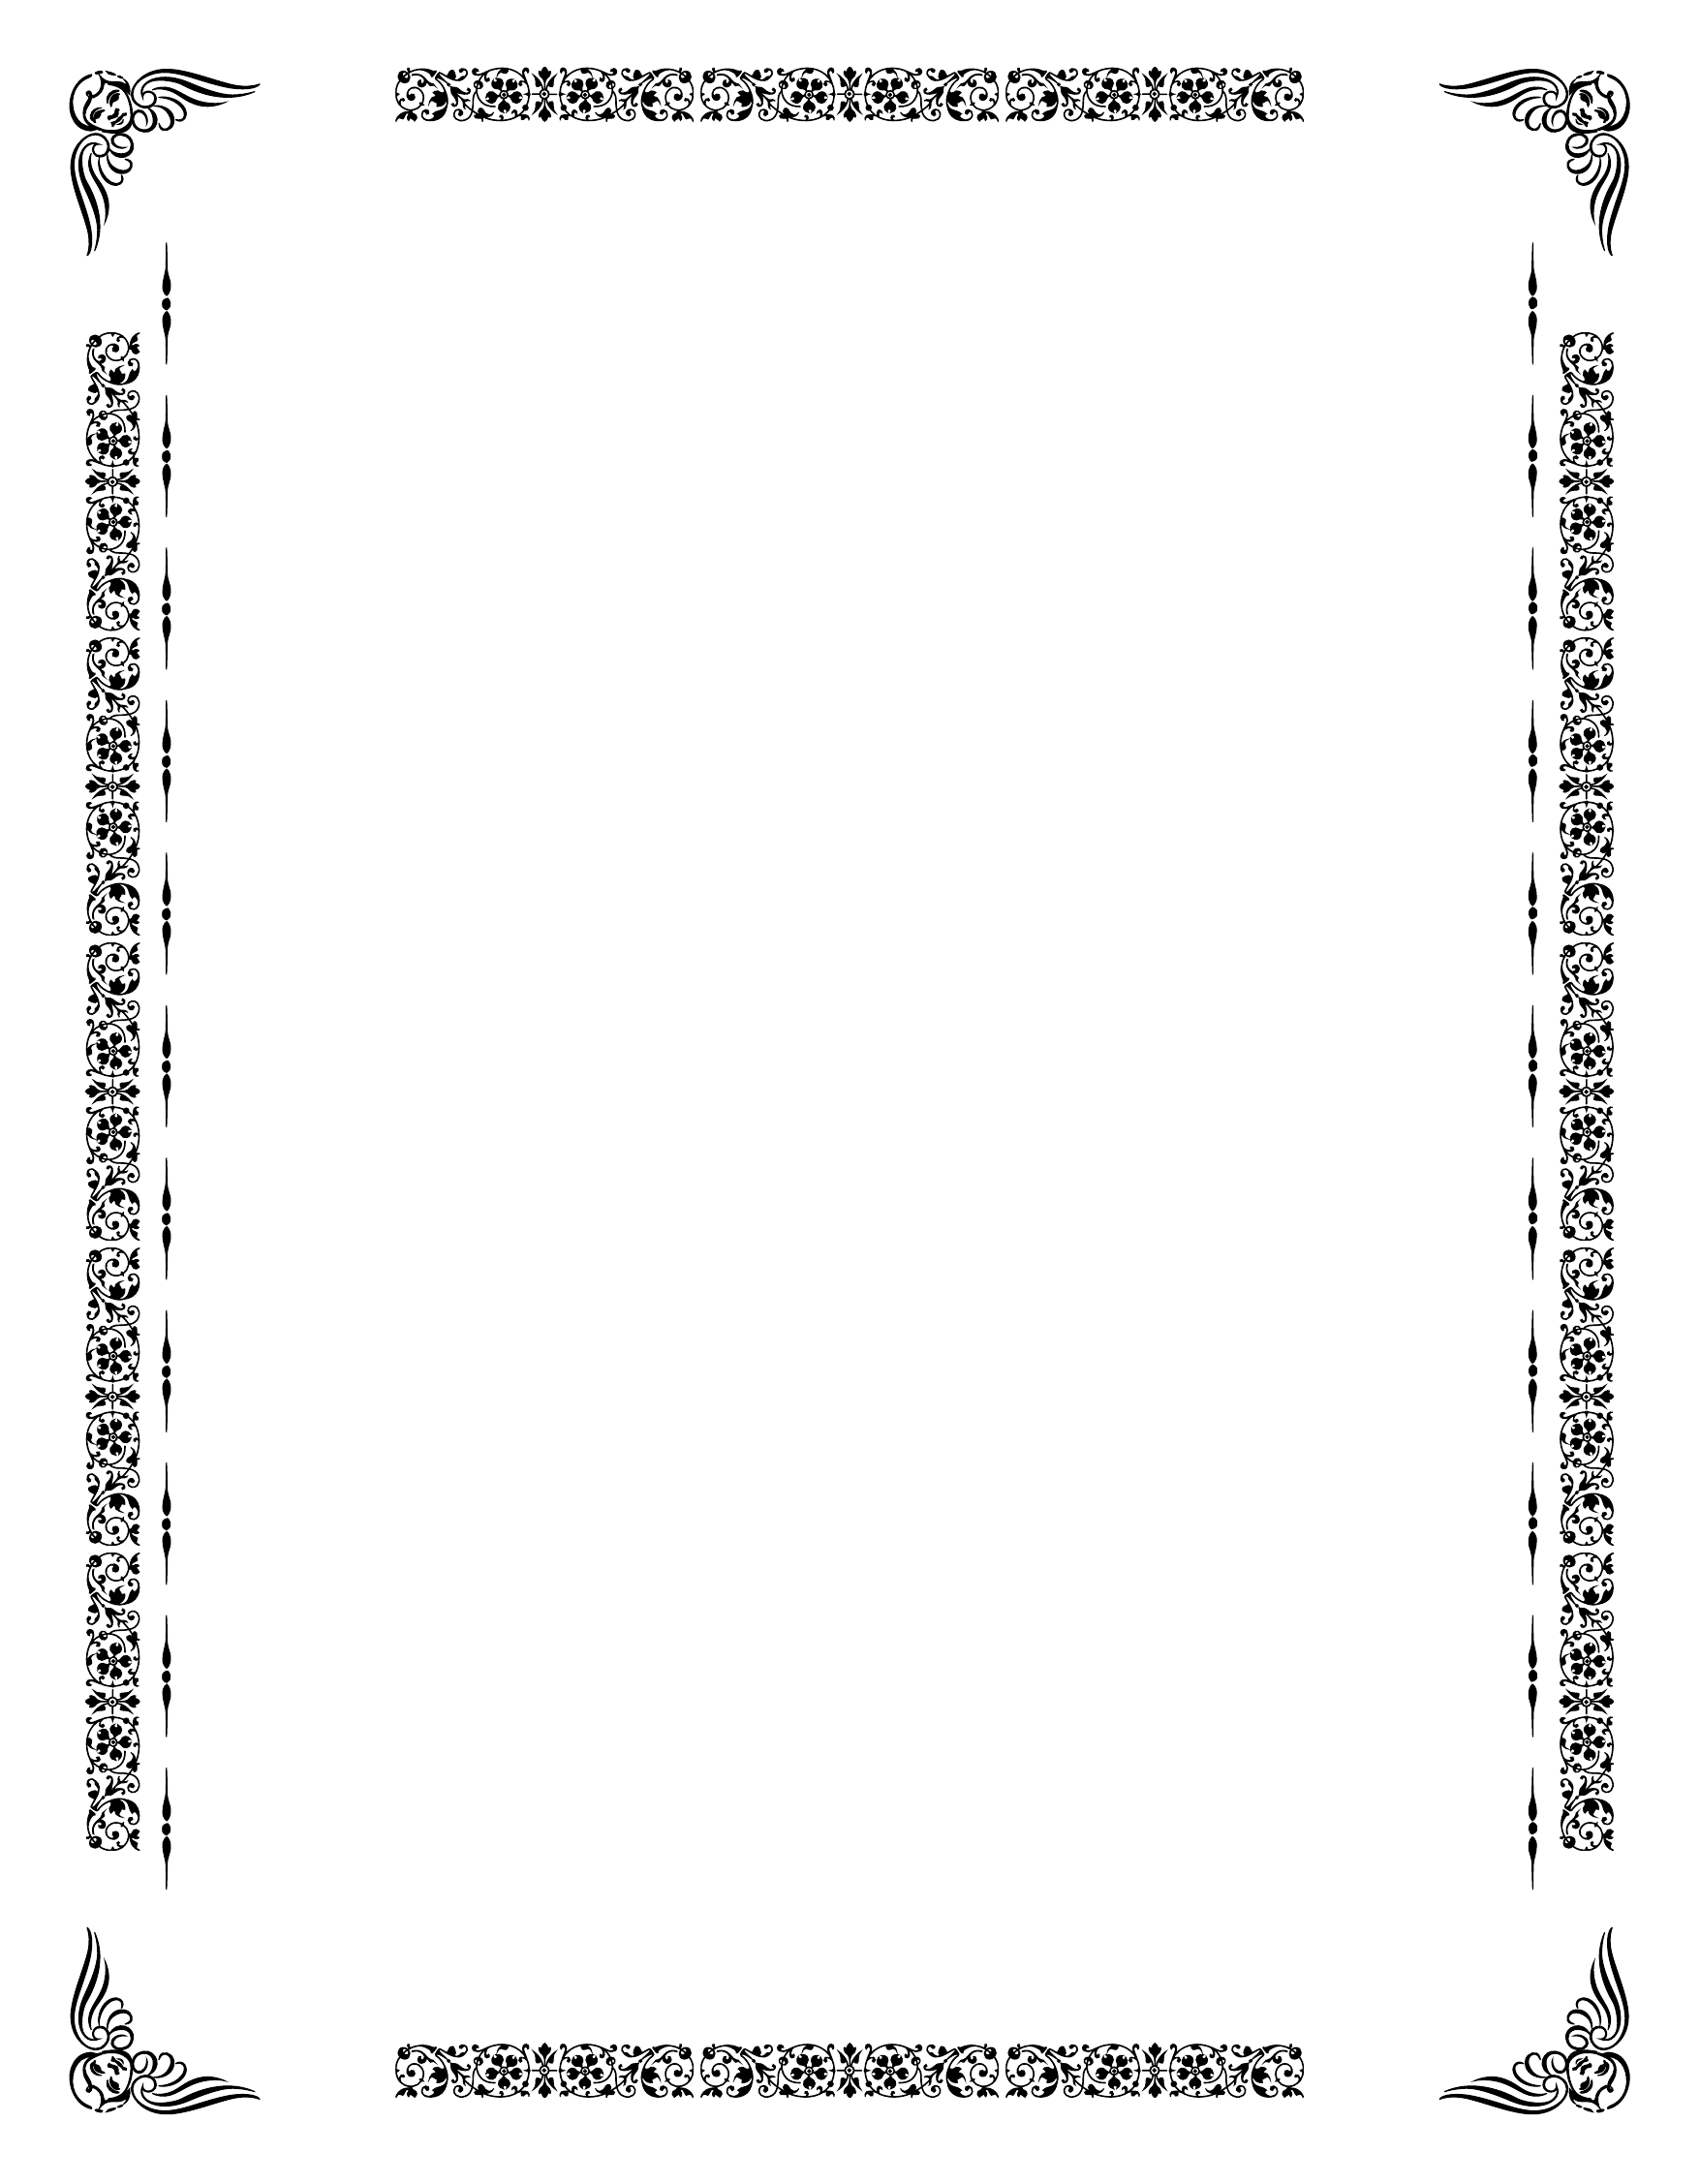
\begin{tikzpicture}[color=black, every node/.style={inner sep= 15pt}]
\node (NW) [anchor=north west] at (current page.north west){\pgfornament[width=2.5cm] {131}};
\node (NE) [anchor=north east] at (current page.north east){\pgfornament[width=2.5cm, symmetry=v]{131}};
\node (SW) [anchor=south west] at (current page.south west){\pgfornament[width=2.5cm, symmetry=h]{131}};
\node (SE) [anchor=south east] at (current page.south east){\pgfornament[width=2.5cm, symmetry=c]{131}};
\foreach \i in {-4,0,4}
\node[anchor=north,xshift=\i cm] at (current page.north){\pgfornament[scale=0.25,symmetry=v]{71}};
\foreach \i in {-4,0,4}
\node[xshift=\i cm, yshift=32.25 pt] at (current page.south){\pgfornament[scale=0.25,symmetry=v]{71}};
\foreach \i in {-8,-4,0,4,8}
\node[yshift=\i cm, xshift=32.25pt, rotate=90] at (current page.west){\pgfornament[scale=0.25,symmetry=v]{71}};
\foreach \i in {-8,-4,0,4,8}
\node[yshift=\i cm, xshift=-32.25pt, rotate=90] at (current page.east){\pgfornament[scale=0.25,symmetry=v]{71}};
\foreach \i in {-11,-9,...,7,9}
\node[anchor=west, yshift=\i cm, xshift=52.25pt, rotate=90] at (current page.west){\pgfornament[scale=0.1]{80}};
\foreach \i in {-11,-9,...,7,9}
\node[anchor=east, yshift=\i cm, xshift=-52.25pt, rotate=-90] at (current page.east){\pgfornament[scale=0.1]{80}};
\end{tikzpicture}
}}

%%%%%%%%%%%%%%%%%%%%%%%%%%%%%%%%%%%%%%%%%%%%%%%%%%%%%%%%%%%%%%%%%%%%%%%%%%%%%%%%%%%%%%%%%%%%%%%%%%%%%%%%%%%%%%%%%%

\centering % Centre everything on the title page
		
\scshape % Use small caps for all text on the title page

\vspace*{\baselineskip} % White space at the top of the page

%------------------------------------------------
%	Title
%------------------------------------------------

\rule{\textwidth}{1.6pt}\vspace*{-\baselineskip}\vspace*{2pt} % Thick horizontal rule
\rule{\textwidth}{0.4pt} % Thin horizontal rule

\vspace{0.75\baselineskip} % Whitespace above the title

{\huge \calligra{ 2025 Spring Math }\\} % Title

\vspace{0.75\baselineskip} % Whitespace below the title

\rule{\textwidth}{0.4pt}\vspace*{-\baselineskip}\vspace{3.2pt} % Thin horizontal rule
\rule{\textwidth}{1.6pt} % Thick horizontal rule

\vspace{2\baselineskip} % Whitespace after the title block

%------------------------------------------------
%	Subtitle
%------------------------------------------------

\LARGE{HTOP,PDE,COMPLEX,ALGO} 

\vspace*{3\baselineskip} % Whitespace under the subtitle



\vspace{0.5\baselineskip} 

{\scshape   \LARGE Yixia Yu\\ } % Editor list

\vspace{0.2\baselineskip} 

\textit{\Large New York University} 

\vfill 

%------------------------------------------------
% Author
%------------------------------------------------

\begin{figure}[!h]
    \centering
    
\includegraphics[width = 5cm, height= 3cm]{resource/image.png}%% include the university icon here
\end{figure}
\vspace{0.3\baselineskip} 


{\large Edited by\\  Yixia Yu\\Email: yy5091@nyu.edu}
\end{titlepage}

\newpage

\backgroundsetup{contents={}} %% to remove background and watermark from other pages
\tableofcontents

%\newpage
\chapter[Algorithm]{Algorithm}
\section[Lecture 1 (02-03) -- {Asymptotic bounds and big O}]{Lecture 1 (02-03)Asymptotic bounds and big O}
\begin{definition}[big-Theta notation(=)]{}
    Let $f,g: N \rightarrow R^+$, we say that $f(n)=\Theta(g(n))$ if there $\exists$  $a,b>0$ and $n_0\in \mathbb{N}$such that $a\cdot g(n) \leq f(n) \leq b\cdot g(n)$ for all $n >n_0$.
    \end{definition}
    Intuitively, $f(n) = \Theta(g(n))$ means that $f(n)$ grows as fast as $g(n)$ up to a constant when $n$ tends to infinity.

    Examples: $3n = \Theta(n)$, $2n^2 + 7n = \Theta(n^2)$, $\ln n^2 = \Theta(\log n)$
\begin{definition}[big-O notation($\leqq$)]{}
    Let $f,g: N \rightarrow R^+$, we say that $f(n)=O(g(n))$ if $\exists$ $n_0\in \mathbb{N} $ and $b>0$  such that $f(n) \leq b \cdot g(n)$ for all $n > n_0$.
    \\ $\lim_{n \rightarrow \infty}sup \frac{f(n)}{g(n)} < + \infty $   
\end{definition}
\begin{definition}[big-Omega notation($\geq$)]{}
    Let $f,g: N \rightarrow R^+$, we say that $f(n)=\Omega(g(n))$ if $\exists$ $n_0\in \mathbb{N} $ and $a>0$  such that $a\cdot g(n)\leq  f(n)  $ for all $n > n_0$.
\\ $\lim_{n \rightarrow \infty}inf \frac{f(n)}{g(n)} >0$
\end{definition}
\begin{remark}{}{}
    $$f(n)=\Theta(g(n)) \Leftrightarrow f(n)=O(g(n)) \text{ and } f(n)=\Omega(g(n))$$
$$f(n)=O(g(n)) \Leftrightarrow g(n)=\Omega(f(n))$$
\end{remark}
\begin{definition}[ittle-o notation(<)]{}
    We write $f(n)=o(g(n))$ if for any $b>0$ there $\exists$ $n_0\in\mathbb{N}$ such that $f(n)<b\cdot g(n)$ for all $n>n_0$.
    \end{definition}
\begin{definition}[little-omega notation(>)]{}
    We write $f(n)=\omega(g(n))$ if for any $a>0$ there $\exists n_0\in\mathbb{N}$ such that $a\cdot g(n)<f(n)$ for all $n>n_0$.
    
\end{definition}
\begin{remark}{}{}
    $f(n)=o(g(n))\Rightarrow f(n)=O(g(n))$ and $f(n)\neq\Theta(g(n))$

$f(n)=\omega(g(n))\Rightarrow f(n)=\Omega(g(n))$ and $f(n)\neq\Theta(g(n))$

$f(n)=\omega(g(n))\Leftrightarrow g(n)=\omega(f(n))$

\end{remark}
$$
    n^{1+\mathrm{e}} , nlog(n) , e \to 0
$$ 
\begin{theorem}{}{}
Any Algorithm has to check at least log(n+1) entries of the sorted array for searching an element in the worst case
\end{theorem}
\section{Recitation 1 (02-07)--{Problem Solving}}
\begin{tabular}{|c|l|c|c|}
    \hline
    \textbf{Notation} & \multicolumn{1}{c|}{\textbf{Bounding Conditions}} & \textbf{Relation} & \textbf{Type} \\ 
    \hline
    $T(n) = O(f(n))$ & $\exists c > 0, \exists n_0, \forall n \geq n_0, T(n) \leq c f(n)$ & $\leq$ & $O$ \\
    \hline
    $T(n) = \Omega(f(n))$ & $\exists c > 0, \exists n_0, \forall n \geq n_0, T(n) \geq c f(n)$ & $\geq$ & $\Omega$ \\
    \hline
    $T(n) = \Theta(f(n))$ & $\exists c_1, c_2 > 0, \exists n_0, \forall n \geq n_0, c_1 f(n) \leq T(n) \leq c_2 f(n)$ & $ = $ & $\Theta$ \\
    \hline
    $T(n) = o(f(n))$ & $\forall c > 0, \exists n_0, \forall n \geq n_0, T(n) < c f(n)$ & $<$ & $o$ \\
    \hline
    $T(n) = \omega(f(n))$ & $\forall c > 0, \exists n_0, \forall n \geq n_0, T(n) > c f(n)$ & $>$ & $\omega$ \\
    \hline
    \end{tabular}
\\
\textbf{Possible useful formula:}
$$
    \int_1^nx^kdx=\frac{n^{k+1}}{k+1}-\frac{1}{k+1}
$$ 
\begin{enumerate}
    \item Multiplication Rule. Prove that for $h(n)=\Omega(1)$, if $f( n)$ = $\Theta ( g( n) )$ then $f(n)\cdot h(n)=\Theta(g(n)\cdot h(n))$ (The same also holds for $O,\Omega,\omega,\omega)$
    \\\textbf{Solution:}
    \begin{align*}  
        &\text{Since } f(n)=\Theta(g(n)), \exists c_1,c_2>0,\exists n_0 \text{ such that }&\\
        &c_1g(n)\leq f(n)\leq c_2g(n),\forall n\geq n_0&\\
         &\text{Since } h(n)=\Omega(1),\text{ there exist constants }c_3>0 \text{ and } n_1 \text{ such that } &\\       
        &h(n)\geq c_3, \forall n\geq n_1&\\
        &\text{Combining the two, we have: }&\\
        &c_1g(n)h(n)\leq f(n)h(n)\leq c_2 g(n)h(n)&\\
        &\text{Therefore } f(n)h(n)=\Theta(g(n)h(n))&
    \end{align*}
    \item Addition Rule.Let $f_{1}, . . . , f_{k}$ : $N$ $\to$ $R_{\geq 0}$ for a fixed number $k$ and $f(n)=$ $\sum_{i=1}^{k}f_{i}(n)$ .Prove that if $f_{i}(n)=O(f_{1}(n))$ for all $i\in\{1,\ldots,k\}$ ,then $f(n)=\Theta(f_{1}(n))$ .Here $f_{1}$ can be replaced with any one of $f_{1},...,f_{k}$
    \\\textbf{Solution:}
    \begin{align*}
        &\text{Since }f_i(n)=O(f_1(n)),\text{ there exist constants }c_i \text{ and } n_0 \text{ such that }&\\
        &f_i(n)\leq c_i f_1(n),\forall n\geq n_0&\\
        &\text{Therefore, }&\\
        &\sum_{i=1}^{k}f_i(n)\leq\sum_{i=1}^{k}c_i f_1(n)=Cf_1(n) \text{ where }C=\sum_{i=1}^{k}c_i &\\
        &\text{Additionally, there exists at least one }f_j(n)=\Omega(f_1(n)),\text{so }\sum_{i=1}^{k}f_i(n)=\Theta(f_1(n))&\\
    \end{align*}
    \item Let $f$ and $g$ be non-negative functions. Define $T(n)=max(f(n),g(n))$ .Prove that $T(n)=\Theta(f(n)+g(n))$
    \\\textbf{Solution:}
    \begin{align*}
        &\text{Since } max(f(n),g(n))\leq f(n)+g(n),\text{ we have } T(n)=O(f(n)+g(n))&\\
        &\text{Also, } f(n)+g(n)\leq 2max(f(n),g(n)),\text{ so } T(n)=\Omega(f(n)+g(n))&\\
        &\text{Therefore, } T(n)=\Theta(f(n)+g(n))&
    \end{align*}
    \item Let $f$ and $g$ be non-decreasing real-valued functions defined on positive integers and $f(1)\geq1$ and $g(1)\geq1$ .Prove or disprove that $f(n)=O(g(n))\Rightarrow2^{f(n)}=O(2^{g(n)})$
    \\\textbf{Solution:}
    \begin{align*}
        &\text{Since } f(n)=O(g(n)),\text{ there exists a constant }c>0 \text{ and } n_0 \text{ such that }&\\
        &f(n)\leq c\cdot g(n),\forall n\geq n_0&\\
        &\text{Therefore, }&\\
        &2^{f(n)}\leq2^{c\cdot g(n)}&\\
        &\text{Since }2^{c}\text{ is constant, we conclude that } 2^{f(n)}=O(2^{g(n)})&
    \end{align*}
    \item Prove that $log(n!)=\Theta(nlogn)$ .Hint:To show an upper bound,compare $n!$ with $n^{n}$ .To show a lower bound, compare it with $\left(\frac{n}{2}\right)^{\frac{n}{2}}$
    \\\textbf{Solution:}
    \begin{align*}
        &\text{We know that: }&\\
        &log(n!)=log(1)+log(2)+\ldots+log(n)&\\
        &\text{Since }log(n) \text{ is increasing, the sum can be bounded by:}&\\
        &log(n!)\leq \sum_{k=1}^{n}log(n)=nlog(n)&\\
        &\text{From the bound, we can use the fact that }log(k)\geq log(\frac{n}{2}) \text{ for all } k\geq2&\\
        &\text{Hence, we can sum the lower half of the terms to get:}&\\
        &log(n!)\geq \sum_{k=\frac{n}{2}}^{n}log(k)\geq \sum_{k=\frac{n}{2}}^{n}log(\frac{n}{2})=\frac{n}{2}log(\frac{n}{2})&\\
    \end{align*}
    \item Show that $c^{n}=o(n!)$ for any constant $C$
    \\\textbf{Solution:}
    \begin{align*}
        &\text{We need to prove that }&\\
        &\lim_{n\rightarrow\infty}\frac{c^n}{n!}=0&\\
        &\text{Using the recursive relation:}&\\
        &\frac{c^n}{n!}=\frac{c^{n-1}}{(n-1)!}\times \frac{c}{n}&\\
        &\text{As }n\rightarrow\infty, \frac{c}{n}\rightarrow0,\text{ Thus, }&\\
        &\lim_{n\rightarrow\infty}\frac{c^n}{n!}=0&\\
    \end{align*}
    \item Show that $c^{n^{1.001}}=\omega(n!)$ for any constant $C$ .Hint: For any fixed numbers $p,q>0$ ,we have $n^{p}=\omega(log^{q}n)$
    \\\textbf{Solution:}
    \begin{align*}
        &\text{We need to prove that }&\\
        &\lim_{n\rightarrow\infty}\frac{c^{n^{1.001}}}{n!}=\infty&\\
        &\text{Taking the algorithm, we have:}&\\
        &log(\frac{c^{n^{1.001}}}{n!})=n^{1.001}log(c)-log(n!)&\\
        &\text{Since }log(n!)\approxeq nlogn,\text{ and }n^1.001 \text{ grows faster than }nlogn,\text{ we conclude that }&\\
        &\lim_{n\rightarrow\infty}log(\frac{c^{n^{1.001}}}{n!})=\infty&\\
        &\text{So,}\lim_{n\rightarrow\infty}\frac{c^{n^{1.001}}}{n!}=\infty&\\
        &\text{Therefore, }c^{n^{1.001}}=\omega(n!)&
    \end{align*}
    \item Show $\sum_{i=1}^ni^k=\Theta(n^{k+1})$ .Hint: Show that $n^{k+1}-(n-1)^{k+1}=\Theta(n^{k})$
    \\\textbf{Solution:}
    \begin{align*}
        &\text{Upperbound: Since }i^k\leq n^k,\text{we have}&\\
        &\sum_{i=1}^ni^k\leq \sum_{i=1}^nn^k=n^{k+1}&\\
        &\text{Lowerbound: Using the integral approximation }&\\
        &\sum_{i=1}^{n}i^k\geq \int_{1}^{n}x^kdx=\frac{n^{k+1}}{k+1}-\frac{1}{k+1}&\\
        &\text{Therefore, }&\\
        &\sum_{i=1}^{n}i^k=\Theta(n^{k+1})&\\
    \end{align*}
    \item Search for the peak. Suppose we have an array $A[1...n]$ and we know that there exists some k (value unknown) such that $A[1]<A[2]<...<A[k]$ and $A[k]>A[k+1]>$ $\ldots>A[n]$ .We call $A[k]$ the peak of $A$ .Design an algorithm to find the peak and analyze it in $O(logn)$ time.
    \\\textbf{Solution:}
    \begin{align*}
        &\text{Use Binary Search Algorithm:}\\
        &\text{1.} \text{Set } l=1,r=n\\
        &\text{2.} \text{While } l<r \text{ do}\\
        &\text{3.} \text{Set } m=\left\lfloor\frac{l+r}{2}\right\rfloor\\
        &\text{4.} \text{If } A[m]<A[m+1] \text{ then } l=m+1\\
        &\text{5.} \text{Else } r=m\\
        &\text{6.} \text{Return } l\\
        &\text{Analysis:}\\
        &\text{Let } T(n) \text{ be the time complexity of the algorithm}\\
        &\text{Let } n_0=1\\
        &\text{Let } c=1\\
        &\text{Let } T(n)=T\left(\frac{n}{2}\right)+c\\
        &\text{Let } T(n)=O(logn)
    \end{align*}
    \item 3SUM in a sorted array.Let $A[1\ldots n]$ be a sorted array. We want to see $A[ i]$ + $A[ j]$ + $A[ k]$ = $x$ for some different $i,j,k$ ,where $x$ is a given number. Design an algorithm $3SUM(n,a,x)$ which can return $(i,j,k)$ or 0 if no such three elements exist.How fast can this problem be solved?
    \\\textbf{Solution:}
    \begin{align*}
        &\text{fix one element A[i], then use two pointers on the remaining array to find } A[j]+A[k]=x-A[i]\\
        &\text{The time complexity is }O(n^2)\\
        &\textbf{Algorithm 3SUM(n,a,x):}\\
        &\text{Input: Array A of n intergers, integer x}\\
        &\text{Output: indices i,j,k such that A[i]+A[j]+A[k]=x or return "No solution" if no such triplet exists}\\
        &\text{for i=0 to n-1 do}\\
        &\text{    //Avoid duplicates by skipping repeated elements}\\
        &\text{    if i>0 and A[i]==A[i-1]}\\
        &\text{        continue}\\
        &\text{    left=i+1,right=n-1}\\
        &\text{    while left<right do}\\
        &\text{        sum=A[i]+A[left]+A[right]}\\
        &\text{        if sum==x}\\
        &\text{            return i,left,right //Found the triplet}\\
        &\text{        if sum<x}\\
        &\text{            left=left+1 //increase the sum by moving left pointer to the right}\\
        &\text{        else}\\
        &\text{            right=right-1 //decrease the sum by moving right pointer to the left}\\
        &\text{return "No solution" //no such triplet exists}\\
    \end{align*}
\end{enumerate}
\section{Recitation 02}

Find tight big-O bounds for the following recurrences (and show your bounds are correct).

Example 1. Substitution. $T(n) = \sqrt{2n} \cdot T(\sqrt{2n}) + \sqrt{n}$ with base case $T(n) = 1$ for $n \in [0,1]$.

Example 2. Recursion Tree. $T(n) = T(n/3) + T(n/4) + T(n/5) + n$

Example 3. Recall The Master Theorem. Let $a \geq 1$, $b > 1$, and $f(n)$ be a function. If $T(n) = aT(n/b) + f(n)$, then we can solve $T(n)$ as:

$$T(n) = \left\{
\begin{array}{ll}
\Theta(n^{log_b a}) & \text{if } f(n) = O(n^{log_b(a-\epsilon)}) \text{ for some } \epsilon > 0 \\
\Theta(n^{log_b a} log n) & \text{if } f(n) = \Theta(n^{log_b a}) \\
\Theta(f(n)) & \text{if } f(n) = \Omega(n^{log_b(a+\epsilon)}) \text{ for some } \epsilon > 0
\end{array}
\right.$$

Then what is the asymptotic bound for: $T(n) = 4T(\frac{n}{2}) + n^2\sqrt{2}$.
\\
Find tight big-O bounds for the following recurrences (and show your bounds are correct).

Problem 1. $T(n) = T(bn) + T(n - bn) + n$, where $b \in (0,1)$ is a constant.
\begin{solution}
    by recursion tree
    \begin{align*}
        H&=log(n)\\
        T(n)&=O(n)\cdot H=O(nlog(n))\\
    \end{align*}
    \end{solution}
Problem 2. $T(n) = n^{\frac{3}{4}}T(n^{\frac{1}{4}}) + n$.
\begin{solution}
    Suppose $ T(n)=C\cdot n^k $ 
    \begin{align*}
        T(m^4)=m^3T(1)+m^4\\
        T(n)=O(n)\\
    \end{align*}
\end{solution}
Problem 3. $T(n) = 2T(2n/3) + T(n/3) + n^2$
\begin{solution}
    by recursion tree
    \begin{align*}
        T(n)&=O(n^2logn)\\
    \end{align*}
\end{solution}
Problem 4. Let $T(n) = 4T(n/3) + n$. Use induction to prove $T(n) = O(n^{log_3 4})$.

Problem 5. $T(n) = T(n-2) + n^2$
\begin{solution}
    \begin{align*}{}{}
    T(n)-T(n-1)&=T(n-2)-T(n-1)+n^2\\
    \text{Let } S(n)&=T(n)-T(n-1)\\
    S(n)&=S(n-1)+n^2\\
    S(n)&=O(n^3)\\
    T(n)&=T(n-1)+O(n^3)\\
    T(n)&=O(n^3)\\
    \end{align*}
\end{solution}
\section{Lecture 2 (02-19) -- {Divide and Conquer}}

\end{document}